\chapter{LoRa}
\section{LoRa}
Tra tutte le tecnologie che cercano di predominare il network layer, LoRaWAN, è
quella che si presta di più alla sperimentazione.
Grazie al protocollo di natura open e la facile reperibilità dei moduli radio e  
sono necessari solo un gateway e dei sensori per creare le prime applicazioni.

\section{Narrow Band e Spread Spectrum}
Il successo delle tecnologie LPWAN risiede nella loro abilità di offrire una
connessione a bassa potenza per un grande numero di devices distribuiti in una
vasta area geografica. Per capire il principio di funzionamento alla base del
layer fisico LoRa, e necessario comprendere il tipo di modulazione utilizzata e
i vantaggi che ne derivano.
Le principali tecniche di modulazione utilizzate dalle reti LPWA sono in grado
di offrire un bilanci di collegamento (link budget ) pari a 150$\pm$ 10[dB], il quale
garantisce un range di operatività pari ad una decina di chilometri.
Andando a ridurre il data rate è possibile concentrare più energia in ogni
simbolo trasmesso. In questo modo il gateway è in grado di decodificare segnali
molto attenuati. In generale le tecnologie LPWAN sono in grado di decodificare
segnali attenuati fino a -130[dBm]. Per ottenere questi risultati due tipi di
modulazione sono stati utilizzati da LPWAN diverse.

\subsection{Narrow Band}
La modulazione narrowband codifica il segnale in una banda molto ristretta (
 $\approx$25[KHz] ), in questo modo è in grado di ottenere alte prestazioni nel
bilancio di collegamento. Assegnando ad ogni frequenza una banda molto
ristretta, la NB è in grado di utilizzare l'intero spettro in maniera efficace.
Il livello di rumore all'interno di ogni canale \improvement{Trovare un termine più
adatto } è molto basso, rendendo semplice la demodulazione da parte del gateway.
Per aumentare la capacità del singolo nodo e diminuire la complessità dei moduli
radio SigFox e altre tecnologie  estremizzano il concetto di narrowband andando a assegnare ad
ogni portante una banda di appena 100[Hz]. Inequivocabilmente il data rate
diminuisce di molto e il tempo il quale il ricevitore deve rimanere acceso
aumenta. 

\subsection{Spread spectrum} 
Come dice il nome, la tecnica spread spectrum è in grado di distribuire un
segnale narrowband in un campo di frequenze più vasto del necessario, mantenendo
però la stessa densità di potenza.
Come risultato otteniamo una trasmissione che incorpora più rumore di una
trasmissione NB, riuscendo però ad essere molto più resistente alle interferenze
ed agli attacchi basati sul jamming.
Per la natura rumorosa del segnale, il ricevitore dovrà compiere uno sforzo
maggiore per la ricezione del segnale, il quale molto spesso sarà ricevuto sotto
il noise floor \improvement{Noise floor in italiano?}
Per ottimizzare l'uso dello spettro, è possibile inviare segnali codificati con
frequenze ortogonali , in questo modo è possibili decodificare in maniera
concorrente segnali diversi, andando ad aumentare la capacità della rete.

\begin{figure}[h]
\centering 
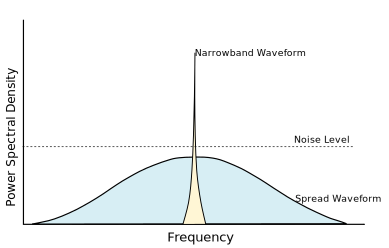
\includegraphics[width=11cm]{spread_spectrum_temp}
\caption{Comparazione tra UNB e SSP}
\end{figure}

\section{CSS}
CSS o Chirp Spread Spectrum è la modulazione alla base del layer fisico LoRa. 
Con Chirp (Compressed High Intensity Radar Pulse) si intende un segnale di
ampiezza costante, il quale incrementa o decrementa la sua frequenza nel tempo.
Parliamo quindi di \emph{UpChirp} nel caso di un aumento di frequenza e di
\emph{DownChirp} nel caso di un decremento.
I l'utilizzo di segnali di tipo Chirp non è nuovo nel campo delle
telecomunicazioni; infatti, questa tecnica di compressione del segnale, 
è molto utilizzata in applicazioni radar o  sonar  poiché tramite essa è possibile aumentare il range
di risoluzione spaziale e il rapporto segnale rumore.
Per aumentare l'efficienza delle sue trasmissioni, LoRa utilizza i segnali Chirp in combinazione ad una
modulazione Spread Spectrum. 
Il più generico segnale chirp è dato dalla equazione \ref{eq:1}
\begin{equation}\label{eq:1}
        s(t) = A\cos(\theta (t))
\end{equation}
possiamo ora definire la frequenza istantanea $f(t)$ \ref{eq:2} ed il parametro
chiamato chirpizzazione istantanea $c(t)$ \ref{eq:3}.
\begin{equation}\label{eq:2}
        \gamma(t) = \frac{1}{2\pi} \frac{d\theta(t)}{dt}
\end{equation}
\begin{equation}\label{eq:3}
        c(t) = \frac{1}{2\pi} \frac{d^2\theta(t)}{dt^2} = \frac{d\gamma(t)}{dt}
\end{equation}
A seconda di come il segnale 
\begin{equation}
        \gamma(t) = \frac{k}{2}t+f_i
\end{equation}
Dove $f_i$ rappresenta la frequenza iniziale del segnale e $k$ la
chirpizzazione.
\begin{equation}
        k = \frac{f_e - f_i}{T}
\end{equation}
con $f_e$ la frequenza finale.
Data una banda $B = [f_0, f_1]$, un segnale di tipo Chirp ha una struttura tale
che, partendo da frequenza iniziale $f_i$, essa verrà incrementa o decrementata
linearmente in modo monotono. Nel caso in cui il segnale raggiunga le frequenze
limite $f_0$ o $f_1$, è necessario far ripartire il segnale dall'estremo opposto
della frequenza raggiunta, in modo da non eccedere la banda di trasmissione e
mantenere la monotonicità.

Con CSS si intende una modulazione che utilizza tutta la banda per l'invio dei
dati.
\begin{figure}[h]
        \centering
                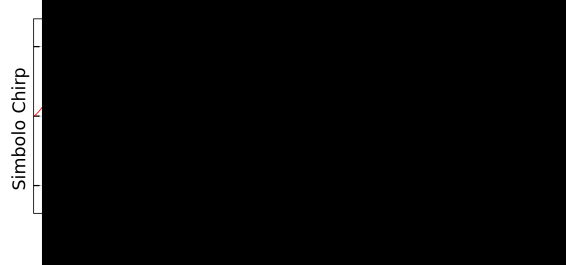
\includegraphics[width=10cm]{Time_Chirp}
        \caption{Esempio di segnale Chirp nel dominio del tempo}
\end{figure}

Come detto in precedenza, il layer fisico LoRa utilizza una modulazione che
prende il nome di Chirp Spread Spectrum. Chirp acronimo di Compressed High
Intensity Radar Pulse, è un segnale  . Questa tipo di modulazione e modulazione è ottenibile facendo
variare in modo lineare la frequenza di un segnale sinusoidale di durata finita
chiamato "Chirp". 
Distribuendo il segnale in un più ampio spettro di quello normalmente richiesto,
e possibile ottenere numerosi vantaggi 
\begin{itemize}
\item Uno spettro idealmente rettangolare, il quale utilizza tutta la capacità
del canale e fornisce un ottima densità spettrale di potenza rispetto agli atri
tipi di trasmissione.
\item \textbf{Segnali di tipo Chirp} possono essere sovrapposti in modo tale da
poter variare il data-rate e l'energia per bit in modo adattativo per aumentare
l'efficienza complessiva.
\item \textbf{Hanno guadagno programmabile}, il quale permette di raggiungere
distanze considerevoli mantenendo un buon SNR .
\item  \textbf{Ottima risoluzione nel asse del tempo}, quindi ottimi per coprire
lunghe distanze.
\item \textbf{Immuni al effetto Doppler} 
\item \textbf{Immuni alle degenerazioni per effetto di multipath} \info{Trovare
termine per multipath}
\end{itemize}
A seconda della scelta di incrementare o decrementare la frequenza, questi
segnali prendono il rispettivo nome di \emph{Up-chirp} o di \emph{down-chirp}.

\begin{figure}[h]
        \centering
                \import{Images/Eps/}{Chirp.eps_tex}
        \caption{Segnale Chirp nel dominio della frequenza}
\end{figure}

Uno degli aspetti peculiari del layer fisico, è la possibilità di andare a
modificare un parametro che prende il nome di SF in modo dinamico per
massimizzare l'efficenza della comunicazione.

do
invariata la potenza impiegata nella trasmissione, di diminuire il bit rate in
modo da aumentare la distanza di trasmissione raggiungibile.
Andando a variare il Spread Factor $SF$ si avranno variazioni sia su

\begin{equation}
        T_s=\frac{2^{\text{SF}}}{B}.
\end{equation}

Dalla quale si evince che andando ad aumentare lo spread factor di una unità,
mantenendo una lunghezza di banda fissa $B$, otteniamo un raddoppio nel tempo di
trasmissione. Il fatto di avere messaggi più lunghi, conferisce un robustezza
superiore alle interferenze e al rumore. In discapito a tutto ciò, il fatto di
dover codificare il messaggio con un maggiore numero di simboli, aumenta la
possibilità di errore alla ricezione. 

\begin{figure}[h]
\centering 
\import{Images/Eps/}{Chirp_SF.eps_tex}
\caption{Comparazione simbolica dei vari SF}
\end{figure}

Questa nuovo modo di trasmettere i vari dati porta con se molti vantaggi.
\begin{itemize}
\item La modulazione Lora è semplice da implementare nei dispositivi, quindi i
moduli radio al loro interno saranno economici.
\item Resistente alle interferenze in banda e fuori banda.
\item Resistente  all'effetto Doppler, in questo modo è possibili utilizzare
cristalli non molto accurati al interno dei devices, in modo tale da abbattere i
costi di produzione.
\item Il modulo di ricezione è altrettanto semplice da costruire, quindi non
molto costoso.
\end{itemize}
\improvement{Rivedere i vari punti e cambiare il linguaggio}

Analizzando lo spettrogramma di una comunicazione Lora è possibile distinguere
in modo semplice le varie parti che compongono il pachetto trasmesso. 

\begin{figure}[h]
\centering 
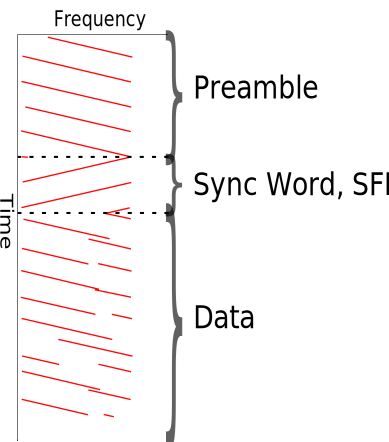
\includegraphics[width=9cm]{Chirp_Message}
\caption{Struttura pacchetto Lora }
\end{figure}

Osservando l'immagine precedente è facile notare come è strutturato un pacchetto.
La prima parte della trasmissione, nonché il preambolo  stesso è codificato con una
serie di \emph{up-chirp}. In questo modo il gateway riesce a sintonizzarsi sulla
stessa frequenza del dispositivo trasmittente.
Successivamente vengono inviati una serie di
\emph{down-chirp} i quali rappresentano l'header codificato dal layer fisico,
dove sono presenti dei bit di controloo e correzzione degli errori
L'ultima parte rappresenta il payload codificato dal PHY, in questa parte,
formata solo da \emph{up-chirp} sono presenti dei salti, i quali sono un chiaro
segno della presenza di dati codificati.

\begin{figure}[h]
\centering 
\includegraphics[width=9cm]{PHY_packet}
\caption{Pacchetto codificato dal layer fisico}
\end{figure}

\improvement[inline]{Aggiungere immagine e finire la spiegazione}

Per quanto riguarda la struttura interna dei moduli radio, non si hanno molte
informazioni dato che la tecnologia è proprietaria di Semtech. Nella
documentazione ufficiale è presente una rappresentazione grafica dei vari
blocchi presenti al interno dei moduli radio.

\begin{figure}[h]
\centering 
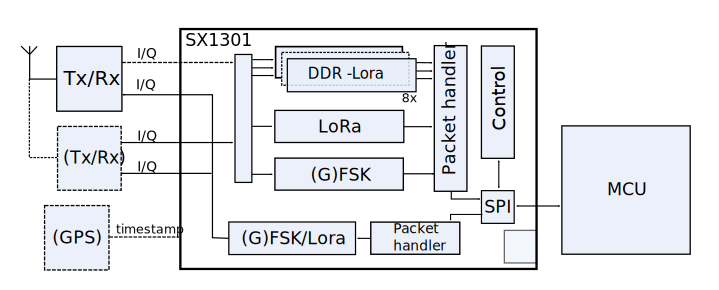
\includegraphics[width=11cm]{SX1301}
\caption{Struttura interna ricevitore SX1301}
\label{fig:sx1301}
\end{figure}

Dalla figura \ref{fig:sx1301} è evidendte che il gateway rimane in ascolto su 8 
frequenze diverse, le quali permettono di coprire tutti i vari SF. 
Tutto ciò è possibili anche grazie al fatto che i vari SF sono quasi ortogonali 
fra di loro, perciò il ricevitore è in grado di ricevere pacchetti da SF diversi 
contemporaneamente. Questo tipo di ricevitore può demodulare fino ad un massimo 
di 8 pacchetti contemporaneamente. Inoltre questa topologia permette di avere 
vari vantaggi
\begin{itemize}
\item I vari nodi della rete, possono cambiare frequenza in ogni trasmissione in
modo casuale, andando a migliorare di molto la robustezza del sistema alle varie
interferenze.
\item Non è necessario avere tabelle contenenti informazioni riguardanti il
data-rate dei vari nodi. Ogni data-rate viene demodulato contemporaneamente.
\item È possibilie utilizzare più antenne nel gateway per realizzare il
cosidetto true antenna diversity, per aumentare la robustezza al multi-path
\end{itemize}
\unsure{Riguardare ultimo punto della documentazione pagina 14}

\section{LoRaWAN}
\info[inline]{Chiedere se il termine protocollo è appropriato}
La parte non proprietaria del protocollo è chiamata \emph{LoRaWAN}, in essa
viene descritta la topologia di rete, la struttura dei pacchetti e le varie
classi di device possibili.

\begin{figure}[h]
\centering 
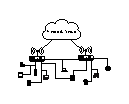
\includegraphics[width=11cm]{LPWAN_Star_network}
\caption{Struttura rete a stella LPWAN}
\end{figure}

La topologia di rete utilizzata, è una topologia a stella, nella quale molti
dispositivi sono connessi e comunicano con uno o più base station. Le BS non
sono altro che dei ponti per poter trasmettere i messaggi ricevuto dai vari
devices all Network Server, tramite una connessione ethernet, 3G o 2G. 
Per come è strutturata la rete, un messaggio inviato
da un singolo device, può essere ricevuto e inoltrato da più BS all Network
Server.

Il NS ha il compito di interpretare e scartare i vari messaggi duplicati che
arrivano, selezionare la BS più adatta per inviare il messaggio di downlink
creando un database di tutti i vari devices presenti nella rete. Nella figura
\ref{fig:stack_lora} è rappresentato lo stack del protocollo degli end-devices,
gateway  e network-server. 

\begin{figure}[h]
\centering 
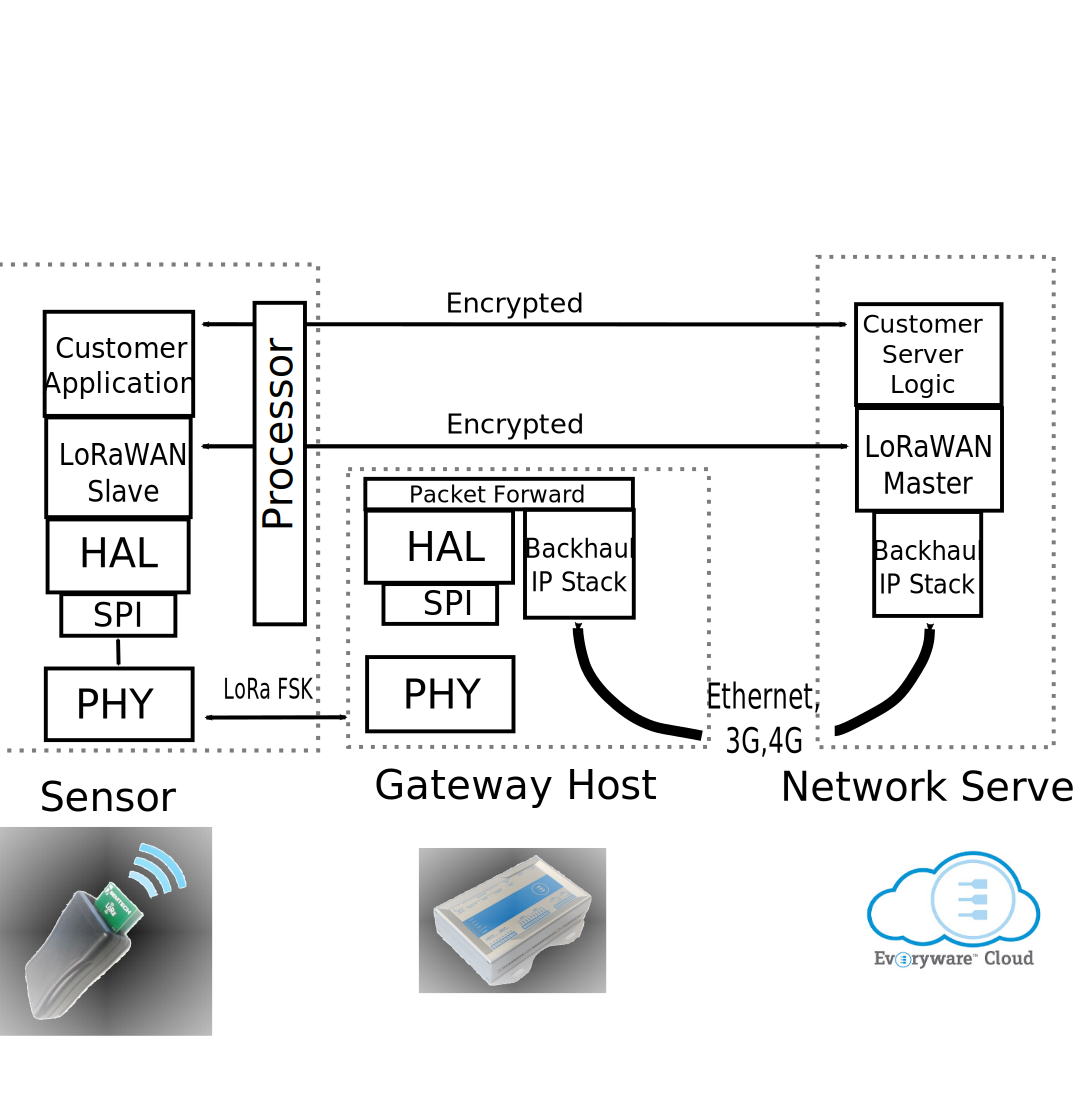
\includegraphics[width=11cm]{Lora_WAN_Stack}
\caption{Stack del protocollo della rete LoRaWAN}
\label{fig:stack_lora}
\end{figure}

Esistono tre classi di devices, le quali specificano i vari use-case per
possibili.

\begin{itemize}
\item \textbf{Class A} è la modalità di funzionamento predefinita. In questa
modalità il device si occupa solo di trasmettere i vari messaggi in maniera
completamente asincrona. Eseguita la trasmissione, due finestre di ascolto
vengono aperte nel end-device. La prima finestra rimane in ascolto nella stessa
frequenza in cui il dato è stato comunicato, mentre la seconda rimane in ascolto
su una frequenza nota a priori e comunicata tramite il MAC.
\item \textbf{Class B} sono devices i quali sono sincronizzati con il NS tramite
beacon packets. In questo modo hanno la possibilità di ricevere dati in un
determinata finestra di tempo. In questa classe rientrano interruttori ,
attuatori ecc..
\item \textbf{Class C} è riservata ai devices che hanno la possibilità di e
essere alimentati direttamente dalla rete elettrica, quindi possono mantenere il
ricevitore costantemente in ascolto.
\end{itemize}

\section{Frequenze}
A seconda della regione in qui operano i devices, lo standard LoRaWAN definisce
 quali frequenze vengono occupate in base alle regolamentazione vigente in
Europa Cina e Stati Uniti.  Per ognuna di queste regioni, vengono definite 
la struttura del payload, la frequenza, lo spreading factor, e la massima
lunghezza possibile del payload.
\begin{table}[h]
        \centering
        \begin{tabular}{l|c}
                \toprule
                Stato   & Frequenza [MHz] \\
                \hline
                Europa  & 868-870 \\
                US      & 902-928 \\
                China   & 779-787 \\
                \bottomrule
        \end{tabular}
        \caption{Bande di frequenza per le varie regioni}
\end{table}
Inoltre tutte le frequenze sono comprese nelle bade ISM, e non sono
particolarmente elevate, rendendole preferibili per le lunghe distanze rispetto
a frequenze quali 2.4 [GHz] e 5[GHz]
